\documentclass{fenicscourse}

\begin{document}

\fenicslecture{Lecture 18: FEniCS C++ programming}
              {Anders Logg}

\begin{frame}
  \frametitle{Two interfaces}

  \textbf{Python}: quick and easy but sometimes slow if
  low-level user-intervention is necessary.

  \bigskip

  \textbf{C++}: potentially faster than the Python interface
  but not for standard problems, requires quite a bit more programming
  expertise.

\end{frame}

\begin{frame}
  \frametitle{Central classes and functions}

  \begin{itemize}
  \item
    \texttt{Mesh}, \texttt{Cell}, \texttt{Vertex}
  \item
    \texttt{Matrix}, \texttt{Vector}, \texttt{LinearSolver}
  \item
    \texttt{Assembler}, \texttt{DirichletBC}
  \item
    \texttt{FunctionSpace}, \texttt{Function}
  \item
    \texttt{LinearVariationalProblem}, \\
    \texttt{LinearVariationalSolver}
  \item
    \texttt{NonlinearVariationalProblem}, \\
    \texttt{NonlinearVariationalSolver}
  \item
    \texttt{assemble}, \texttt{solve}
  \end{itemize}

  \bigskip

  But no \texttt{dot}, \texttt{grad} or \texttt{dx}!

\end{frame}

\begin{frame}
  \frametitle{Code generation}

\begin{center}
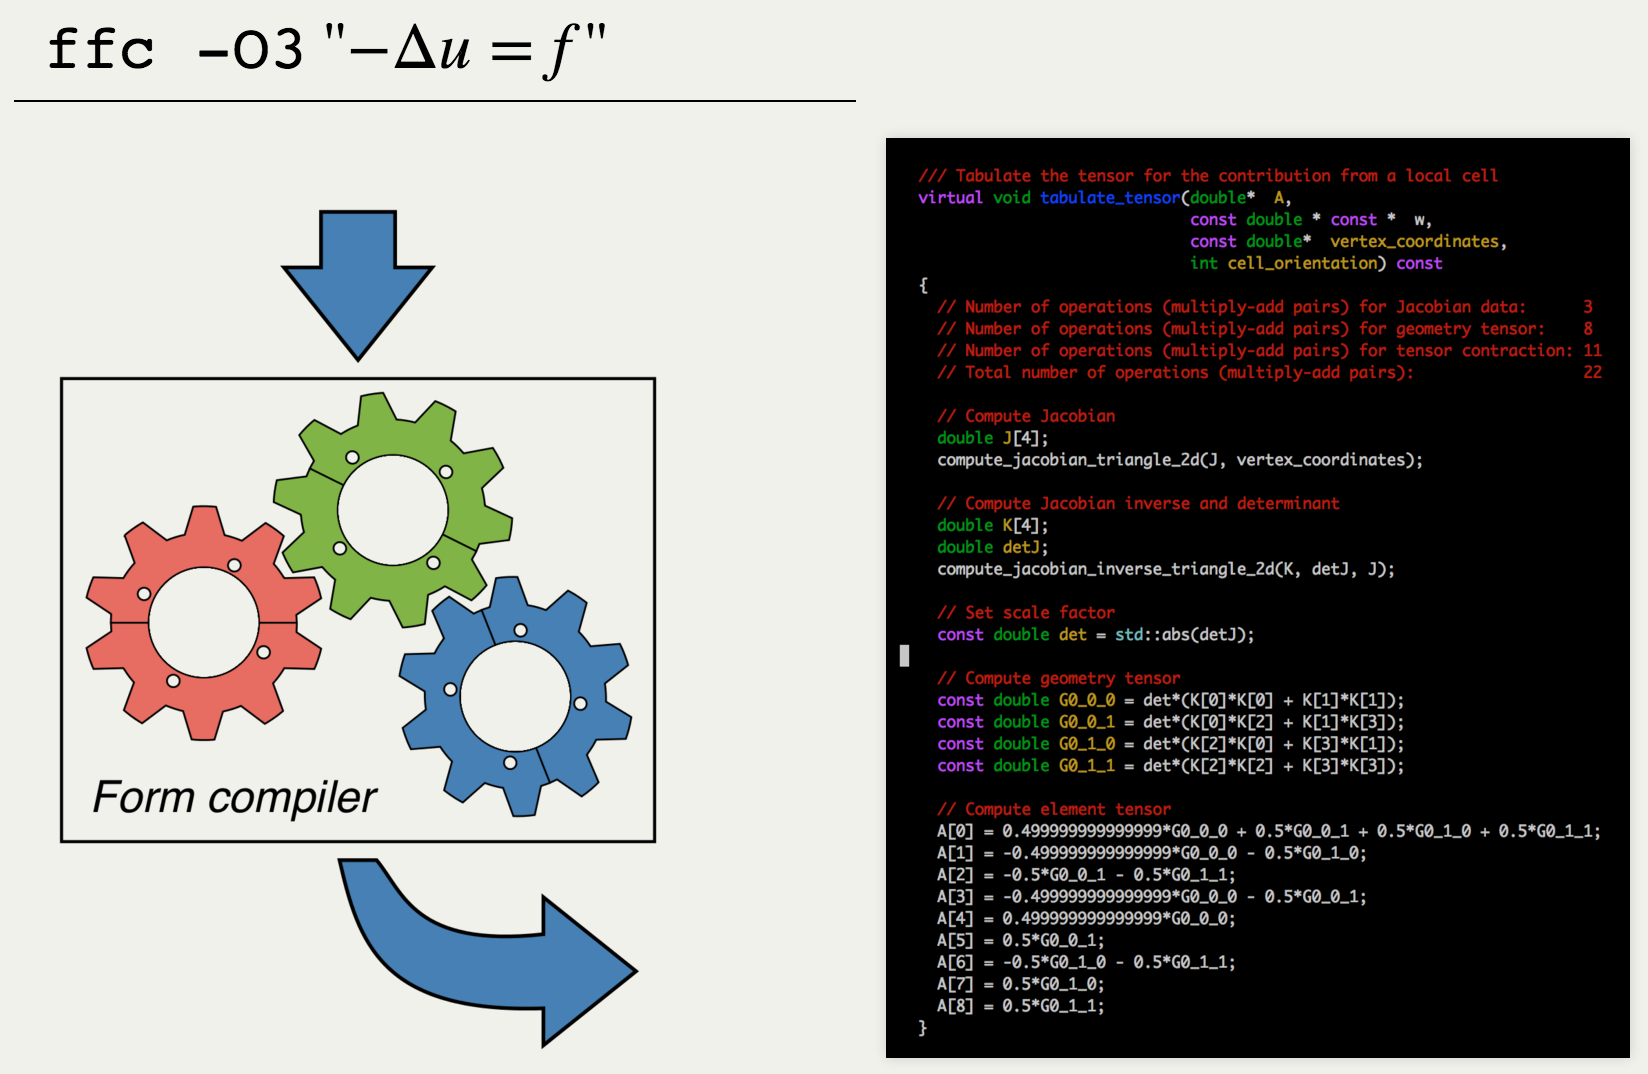
\includegraphics[width=\textwidth]{png/codegeneration_new.png}
\end{center}

\end{frame}

\begin{frame}[fragile]
  \frametitle{Writing a form file}

\begin{python}
element = FiniteElement("Lagrange", triangle, 1)

u = TrialFunction(element)
v = TestFunction(element)
f = Coefficient(element)

a = dot(grad(u), grad(v))*dx
L = f*v*dx
\end{python}

\bigskip

Similar to Python (and UFL is actually a Python extension).

\bigskip

Replace \texttt{FunctionSpace} by \texttt{FiniteElement}.

\end{frame}

\begin{frame}[fragile]
  \frametitle{Calling the form compiler}

\begin{bash}
ffc -l dolfin MyForms.ufl
\end{bash}

\bigskip

This generates \texttt{MyForms.h} from \texttt{MyForms.ufl}.

\bigskip

Type \texttt{man fcc} for command-line options (such as optimizations).

\end{frame}

\begin{frame}[fragile]
  \frametitle{Including forms}

  \begin{c++}
#include "MyForms.h"

int main()
{
  ...

  MyForms::BilinearForm a(V, V);
  MyForms::LinearForm L(V);

}
  \end{c++}

Define forms in \texttt{.ufl} file. \\
Generate C++ code using FFC. \\
Include generated C++ code in C++ program. \\
Instantiate form objects in C++ program.

\end{frame}

\begin{frame}[fragile]
  \frametitle{Attaching coefficients}

\begin{c++}
L.f = f;

L.set_coefficient(0, f);

L.set_coefficient("f", f);

L.set_coefficients(...);
\end{c++}

  \bigskip

  A \texttt{Coefficient} is either an
  \texttt{Expression}, a
  \texttt{Constant} or a
  \texttt{Function}.

\end{frame}

\begin{frame}[fragile]
  \frametitle{Assembly and solve}

\begin{c++}
assemble(A, a);
assemble(b, L);
\end{c++}

\bigskip

\begin{c++}
solve(a == L, u, bc);
solve(F == 0, u, bc, J);
\end{c++}

\end{frame}


\begin{frame}[fragile]
  \frametitle{Using shared pointers}

  \begin{c++}
Mesh* mesh = new Mesh(); // raw pointer
delete mesh;             // delete necessary
  \end{c++}

  \begin{c++}
std::shared_ptr<Mesh> mesh(new Mesh())
  \end{c++}

  \begin{c++}
auto mesh = std::make_shared<Mesh>();
  \end{c++}

\bigskip

Some FEniCS (DOLFIN) C++ functions expect
a shared pointer, while others expect a reference.

\end{frame}

\begin{frame}[fragile]
  \frametitle{Building the program (hard option)}

\begin{code}
cmake_minimum_required(VERSION 3.5)

set(PROJECT_NAME demo_poisson)
project(${PROJECT_NAME})

# Set CMake behavior
cmake_policy(SET CMP0004 NEW)

# Get DOLFIN configuration data
find_package(DOLFIN REQUIRED)
...

# Add executable
add_executable(${PROJECT_NAME} main.cpp)

# Target libraries
target_link_libraries(${PROJECT_NAME} ${DOLFIN_LIBRARIES})
\end{code}

\end{frame}

\begin{frame}[fragile]
  \frametitle{Building the program (easy option)}

  \begin{itemize}
  \item
    Copy \texttt{CMakeLists.txt} from one of the DOLFIN demos
  \item
    Edit: add source files and rename executable
  \item
    Make an out-of-source build:
  \end{itemize}

  \begin{c++}
mkdir build
cd build
cmake ..
make
./myprogram
  \end{c++}

\end{frame}

\begin{frame}
  \frametitle{Solving Poisson's equation}

  We return to the simple Poisson equation and investigate how
  to write a FEniCS C++ solver:
  \begin{alignat*}{2}
      - \Delta u &= f \,\,\, \quad &&\mbox{in } \Omega
      \\
    u &= u_0 \quad &&\mbox{on } \Gamma_D \\
    \partial u/\partial n &= g \quad &&\mbox{on } \Gamma_N \\
  \end{alignat*}
  We will take
  \begin{equation*}
    f(x, y) = 10\cdot\exp(-((x-0.5)^2 + (y-0.5)^2)/0.02)
  \end{equation*}

\end{frame}

\begin{frame}
  \frametitle{Variational problem}

  Find $u \in V$ such that
  \bigskip
  \begin{equation*}
    \int_{\Omega} \nabla u \cdot \nabla v \dx =
    \int_{\Omega} f v \dx + \int_{\Gamma_N} g v \ds
  \end{equation*}

  \bigskip
  for all $v \in \hat{V}$

\end{frame}

\begin{frame}[fragile]
  \frametitle{Form file: \texttt{Poisson.ufl}}

\begin{python}
element = FiniteElement("Lagrange", triangle, 1)

u = TrialFunction(element)
v = TestFunction(element)
f = Coefficient(element)
g = Coefficient(element)

a = inner(grad(u), grad(v))*dx
L = f*v*dx + g*v*ds
\end{python}

\end{frame}

\begin{frame}[fragile]
  \frametitle{Calling the form compiler}

\begin{bash}
ffc -l dolfin Poisson.ufl
\end{bash}

\bigskip

This generates \texttt{Poisson.h} from \texttt{Poisson.ufl}.

\end{frame}

\begin{frame}[fragile]
  \frametitle{C++ implementation: \texttt{main.cpp} (1/3)}

\begin{c++}
#include <dolfin.h>
#include "Poisson.h"

using namespace dolfin;

class Source : public Expression
{
  void eval(Array<double>& values,
            const Array<double>& x) const
  {
    double dx = x[0] - 0.5;
    double dy = x[1] - 0.5;
    values[0] = 10*exp(-(dx*dx+dy*dy)/0.02);
  }
};
\end{c++}

\end{frame}

\begin{frame}[fragile]
  \frametitle{C++ implementation: \texttt{main.cpp} (2/3)}

\begin{c++}[basicstyle=\scriptsize]
int main()
{
  auto mesh =
   std::make_shared<UnitSquareMesh>(32, 32);
  auto V
   std::make_shared<Poisson::FunctionSpace>(mesh);
  auto u0 =
   std::make_shared<Constant>(0.0);
  auto boundary =
   std::make_shared<DirichletBoundary>();

  DirichletBC bc(V, u0, boundary);

  Poisson::BilinearForm a(V, V);
  Poisson::LinearForm L(V);

  auto f = std::make_shared<Source>();
  auto g = std::make_shared<dUdN>();
  L.f = f;
  L.g = g;
\end{c++}

\end{frame}

\begin{frame}[fragile]
  \frametitle{C++ implementation: \texttt{main.cpp} (3/3)}

\begin{c++}
  Function u(V);
  solve(a == L, u, bc);

  File file("poisson.pvd");
  file << u;

  plot(u);

  interactive();

  return 0;
}
\end{c++}

\end{frame}

\end{document}
